\documentclass{article}

\usepackage{amsthm}
\usepackage{amsmath}
\usepackage{amssymb}
\usepackage{graphicx}

\title{CS3410 Project 1 Design Document}
\date{February 25, 2015}
\author{Alexandra Anderson, Joshua Hull}

\begin{document}
\maketitle

\section*{Introduction}
Our MIPS processor will follow a five stage pipeline as discussed in class.  Each stage will be blocked off with registers storing necessary data.  Instructions will proceed through one stage of the pipeline per clock cycle. The overall diagram of how the stages are laid out is as follows:

\begin{figure}[h]
	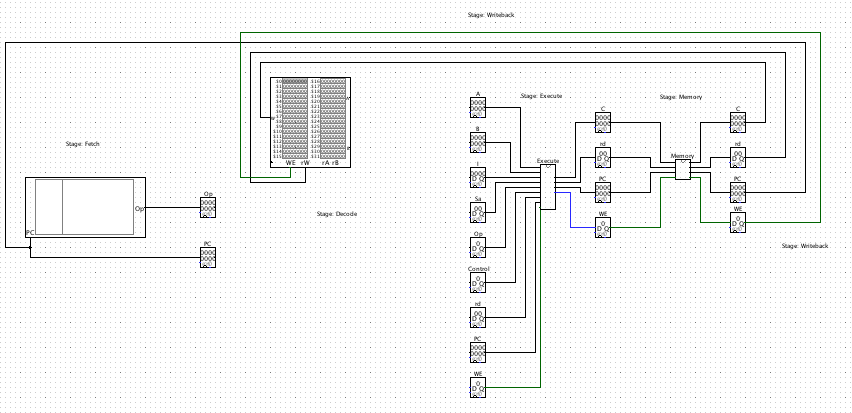
\includegraphics[width = \textwidth]{layout}
	\caption{The layout of the MIPS pipeline in five stages.}
\end{figure}

This is merely a design diagram. While we will implement the pipeline processor in the overall layout and sub circuits shown, very few wires are currently connected. The fetch, decode, and execute stages are not yet implemented, although space for them has been allocated. 

\section*{Fetch}
This stage Fetches the next instruction from the instruction memory and updates the program counter.  Both the instruction and PC$+4$ are passed into the register so that the next stage (Decode) has access to that information.  

This stage also includes a multiplexer to select between PC$+4$ and jump/branch targets.

\section*{Decode}
This stage uses the bits in the instruction to determine several different values:

It determines the immediate value for immediate operations (this value is computed regardless of whether or not the operation is an immediate operation - it is selected for using a multiplexer in the next stage).

It determines which registers to read from (and reads those registers).

It determines a shift amount and op-code to send to the ALU.

It also determines jump and branch amounts (though these values are not used).

The registers at the end of this stage will store certain data for the next stage including the values of the read registers, PC$+4$, jump and branch targets, the immediate value, the shift amount, the op code, the write enable bit, and the register to write to. There are also two extra control bits indicating the presence of a set less than operation and whether it is signed or unsigned, and one more indicating whether this is an immediate or register operation. 

\section*{Execute}
This section sign-extends the immediate value and selects whether to use register B or the immediate value in the operation.  Then, it performs the given ALU operation.

This result is then combined with some additional logic (comparators in the case of SLT for instance) and the result of the operation is outputted.

To implement the comparators SLTI and SLTIU, we can use the ALU subtraction operation. We separate out the MSB's of A and B, and compare them. If they are different, we have an immediate answer. If they are the same, we look to the output of the ALU. By replacing the sign bit with a 0, we preserve the ordering of the distinct sets $\{x \geq 0\}$ and $\{x < 0\}$. 

Then the result of the subtraction operation will have a sign bit of either 1 or 0. If the sign bit is 1, then we know $A < B$, and if the sign bit is 0, we know $A \geq B$, provided that the original MSB's of A and B, either signed or unsigned, were the same. 

The registers at the end of this stage will store PC$+4$, jump and branch targets, the result of the ALU operation, the write enable bit, and the register to write to.

\section*{Memory}
This section will be a pass-through stage. There will not be any logic here, though it will be blocked off by registers so all operations have to spend a cycle in this stage. The registers at the end of this stage store the same values as the registers at it's beginning, for Project 1. 

\section*{Writeback}
This section will only write the results of the register and immediate operations that we have to implement.  It will not write the bits read from memory (as these operations will not be implemented).

\end{document}